% This is an example to show the beamer template NewLuebeck.
\documentclass[9pt]{beamer}

% Alternatively you can use the article mode to print a handout
%\documentclass{article}
%\usepackage{beamerarticle}

\usepackage[T1]{fontenc}                    % Ausgabekodierung
\usepackage[utf8]{inputenc}                 % Eingabekodierung
\usepackage[english]{babel}               % English 
\usepackage{graphicx}
\usepackage{url}
\usepackage{hyperref}
\usepackage{listings}
\usepackage{caption}
\usepackage{multicol}
\usepackage{listings}
\usepackage{tikz}
\usetikzlibrary{calc,patterns,decorations.pathmorphing,decorations.markings,}
\setbeamertemplate{caption}[numbered]


\mode<presentation>{
\usetheme{NewLuebeck}
\title{Web Servers}
\author[Richter]{Markus Richter}
\institute{Institute for Software Engineering and Programming Languages}
\subject{Beispiel}
\keywords{Web servers}
}

\mode<article>{
\usepackage{document}
\documentAuthors{Markus Richter}
\documentTerm{WS 2013}
\documentDate{\today}
\documentTitle{Web Servers}
}

\lstset{% 
numbers=left, numberfirstline=true,
basicstyle=\ttfamily,
showstringspaces=false
}%

\begin{document}
\frame{\titlepage}
\mode<article>{\printDocumentHeader}

\begin{frame}
\frametitle<presentation>{Table of Contents}
\tableofcontents
\end{frame}

\section{Introduction}
\begin{frame}
\frametitle<presentation>{}
  \begin{alertblock}{It's not a bug!}
  The terms Web and Internet are proper nouns and thus are capitalized!
  \end{alertblock}
\end{frame}

\begin{frame}
\frametitle<presentation>{Introduction}
  \begin{itemize}
    \item The Internet is growing
    \item Not for information gain only
    \item Services for business, communication, entertainment
    \item Key to the success of the Internet
  \end{itemize}
  $\Longrightarrow$  Made possible by Web servers
\end{frame}


\begin{frame}
\frametitle<presentation>{Introduction}
As Web servers play an important role

\begin{enumerate}
  \item How to support development of Web sites towards more attractive and modern Web sites?
  \item How to assure high performance in the Web?
\end{enumerate}

\end{frame}

\section{Definitions}
\begin{frame}
  \frametitle<presentation>{Definitions - Web server}

  \begin{figure}[h]
    \centerline{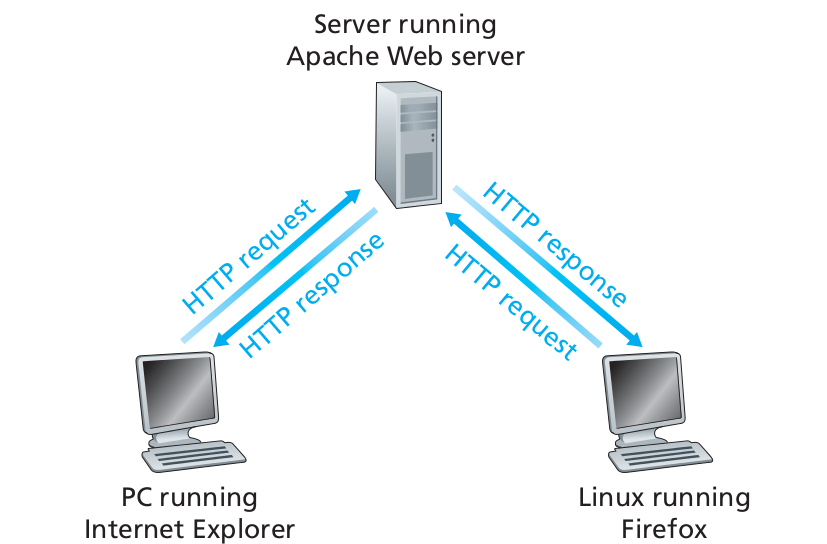
\includegraphics[width=8cm]{pics/client_server.png}}
    \caption{Client Server Architecture. Taken from \cite{kurose}}
  \end{figure}
  
\end{frame}

\begin{frame}
 \frametitle<presentation>{Definitions - HTTP}
    \begin{itemize}
    \item HyperText Transfer Protocol
    \item Application-layer protocol
    \item Server Client Architecture
    \item Communication by using HTTP messages
  \end{itemize}
\end{frame}

\section{Concept}
\begin{frame}
 \frametitle<presentation>{Concept}
 
 \begin{multicols}{2}
    \begin{itemize}
      \item Mainly based on HTTP
      \item Communication by using HTTP messages
      \item Static behaviour
    \end{itemize}
  
   Files addressed by URL:
    \begin{itemize}
      \item HTML files
      \item jpg, png, pdf etc.
      \item $\hdots $
    \end{itemize}
  \end{multicols}
  
  \begin{figure}[h]
    \centerline{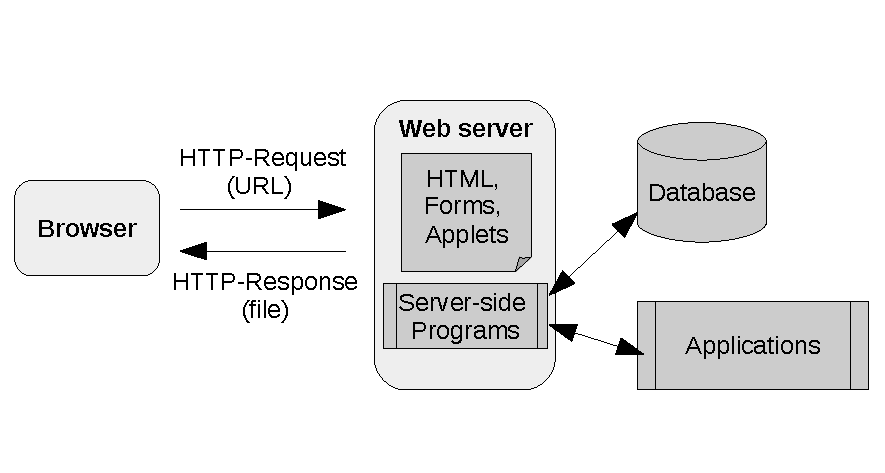
\includegraphics[width=8cm]{pics/webclient.pdf}}
    \caption{Concept of an HTTP Web server}
    \label{fig-webserverconcept}
  \end{figure}

\end{frame}

\begin{frame}[fragile]
 \frametitle<presentation>{Example HTTP - Request}
  \begin{exampleblock}{Example}
    \begin{lstlisting}[mathescape, captionpos=b,caption={Simple HTTP request message. Taken from \cite{kurose}},label=lst:httpRequest]
      GET /somedir/page.html HTTP/1.1
      Host: www.someschool.edu
      Connection: close
      User-agent: Mozilla/5.0
      Accept-language: fr
    \end{lstlisting}
  \end{exampleblock}
\end{frame}

\begin{frame}[fragile]
\frametitle<presentation>{Example HTTP - Response}
  \begin{exampleblock}{Example}
    \begin{lstlisting}[mathescape, captionpos=b,caption={Simple HTTP response message. Taken from \cite{kurose}},label=lst:httpResponse] 
      HTTP/1.1 200 OK
      Connection: close
      Date: Tue, 09 Aug 2011 15:44:04 GMT
      Server: Apache/2.2.3 (CentOS)
      Last-Modified: Tue, 09 Aug 2011 15:11:03 GMT
      Content-Length: 6821
      Content-Type: text/html

      (data data data data data $\hdots$)
    \end{lstlisting}
  \end{exampleblock}

\end{frame}

\section{History}
\begin{frame}
\frametitle<presentation>{History}

  \begin{itemize}
    \item Closely tied to the history of the Internet
    \item Web servers still rely on HTTP and HTML 
  \end{itemize}
  
  \begin{center}  
   \begin{figure}[h]
    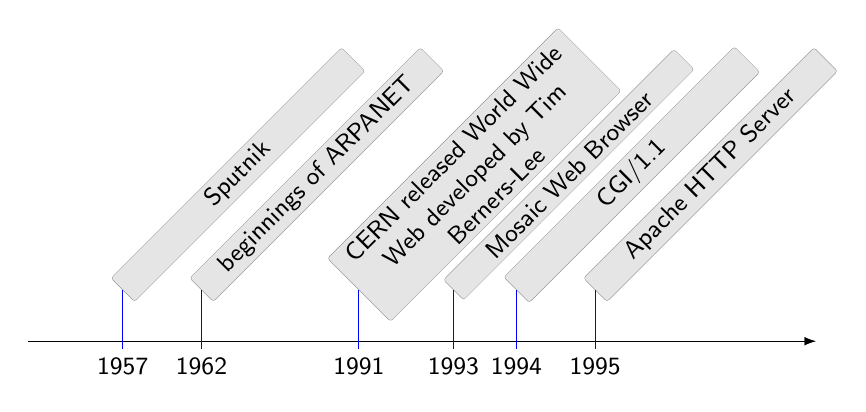
\begin{tikzpicture}[scale=1]
      \small \sf 
      \tikzset{label/.style={draw=gray, ultra thin, rounded corners=.25ex, fill=gray!20,text width=4cm, text badly centered,  inner sep=.5ex, above = 2em, anchor=west,rotate=45}}
      \tikzset{tick/.style={below=3pt}}
      \tikzset{thinline/.style={ultra thin}}
      \draw (0,0) -- (6,0);
      %draw arrow 
      \draw (0,0)[->, -latex] -- (10,0);
      %draw 
      \draw (0,0)[->, -latex] -- (10,0);
      %draw vertical lines
      %\foreach \x in {1.2,2.2,4.2,5.2,6.2,8.2,9.2,10.2} 
      %               \draw (\x cm,2ex) node (\x) {*};
      %draw nodes
      \draw (1.2,0) node (A0) [tick] {1957} node (B0)[label] {Sputnik};
      \draw (2.2,0) node(A1) [tick] {1962} node (B1) [label]  {beginnings of ARPANET};
      \draw (3.2,0) node (A2) [tick] {$\hdots$} node (B2) {};
      \draw (4.2,0) node[tick] (A3) {1991} node (B3) [label] {CERN released World Wide Web developed by Tim Berners-Lee};
      \draw (5.4,0) node[tick] (A4) {1993} node (B4) [label]  {Mosaic Web Browser};
      \draw (6.2,0) node[tick] (A5) {1994} node (B5) [label] {CGI/1.1};
      \draw (7.2,0) node[tick] (A6) {1995} node (B6) [label] {Apache HTTP Server};
      \draw (8.2,0) node[tick] (A7) {} node (B7) []  {};

      \foreach \nn in {0,1,3,4,5,6}
      {   \draw[blue] (B\nn.west) -- ++(0,-0.75);
      }

      \end{tikzpicture}
      \caption{Chronology of the Web}
    \end{figure}
  \end{center}
\end{frame}

\section{Server-side Technologies}
\begin{frame}
\begin{multicols}{2}
\frametitle<presentation>{Server-side Technologies}
  \begin{itemize}
    \item Need for interactivity grew
    \item Number of competing technologies evolved
    \item Used as external programs or modules
    \item Examples: CGI, ASP.NET, PHP, JSP
  \end{itemize}
  
  \begin{figure}[h]
    \centerline{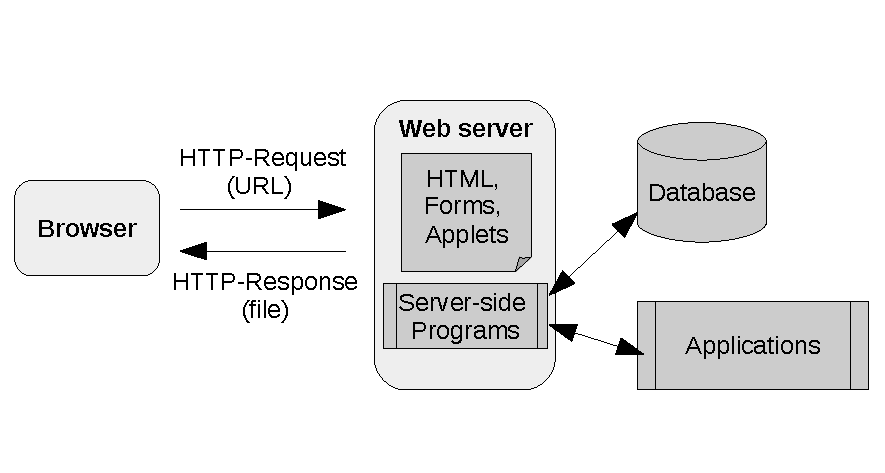
\includegraphics[width=6cm]{pics/webclient.pdf}}
  \end{figure}
\end{multicols}

\end{frame}

\begin{frame}
\frametitle<presentation>{CGI - Common Gateway Interface}
  \begin{block}{Definition \cite{cgiSpecs}}
    A simple interface for running external programs, software or gateways under an information server in a platform-independent manner
  \end{block}

  \begin{figure}[h]
    \centerline{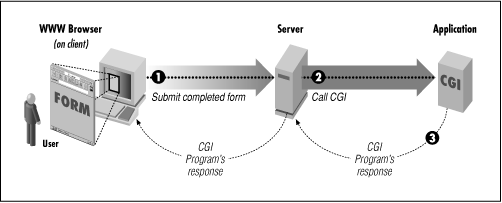
\includegraphics[width=8cm]{pics/cgi.png}}
    \caption{How CGI works. Taken from \cite{gundavaram1996cgi}}
    \label{fig-cgi}
  \end{figure}

\end{frame}

\begin{frame}[fragile]
\frametitle<presentation>{CGI - Common Gateway Interface}

  \begin{exampleblock}{Example}
    \begin{lstlisting}[captionpos=b,caption={Client request for CGI program. Taken from \cite{gundavaram1996cgi}},label=lst:cgiProgram]
      GET /cgi-bin/welcome.pl HTTP/1.0
      Accept: www/source
      Accept: text/html
      Accept: image/gif
      User-Agent: Lynx/2.4 libwww/2.14
      From: shishir@bu.edu
    \end{lstlisting}
  \end{exampleblock}
\end{frame}

\begin{frame}
  Result of execution can be
  
  \begin{itemize}
    \item a new document 
    \item an URL to an existing one
  \end{itemize}
  
  \frametitle<presentation>{CGI - Common Gateway Interface}

  
  \begin{multicols}{2}
     Advantages:
     \begin{itemize}
       \item CGI is platform-independent 
     \end{itemize}
     \vfill
     \columnbreak 
     
    Significant drawbacks:
    \begin{itemize}
      \item Low scalability
      \item Bad performance
    \end{itemize}
  \end{multicols}
    
  $\Longrightarrow $ Most modern Web servers provide their own solutions for popular technologies, e.g. \emph{mod\_php}, \emph{mod\_perl} for Apache.
  
\end{frame}

\begin{frame}
\frametitle<presentation>{PHP:Hypertext Preprocessor}
  \begin{block}{Definition \cite{PHPPreface}}
  A widely-used Open Source general-purpose scripting language that is especially suited for Web development and can be embedded into HTML. Its
  syntax draws upon C, Java, and Perl, and is easy to learn.
  \end{block}
  
  \begin{itemize}
  \item According to \cite{w3TechsStats} by far the most popular used technology in Web development
  \item Needs to be interpreted
  \item Interpreter can be a module or a CGI binary
  \item Embedded inside HTML and executed every time the HTML file is accessed
  \item Usually used together with Linux, Apache Web server, MySQL (LAMP architecture)
  \end{itemize}
  
\end{frame}

\begin{frame}[fragile]
\frametitle<presentation>{PHP:Hypertext Preprocessor}

  \begin{exampleblock}{Example}
    \begin{lstlisting}[language=php, captionpos=b,caption={PHP embedded in HTML. Taken from \cite{welling2008php}},label=lst:php]
      <?php
      echo "<p>Order processed at ";
      echo date('H:i, jS F Y');
      echo "</p>";
      ?>
    \end{lstlisting}
  \end{exampleblock}
\end{frame}

\begin{frame}
\frametitle<presentation>{PHP:Hypertext Preprocessor}

  \begin{multicols}{2}
    Advantages of PHP:
    \begin{itemize}
    \item High performance
    \item High scalability
    \item Object oriented support
    \item Database integration
    \item Low costs
    \end{itemize}
    
    Disadvantages:
    \begin{itemize}
      \item Code maintenance 
      \item Not fully object oriented
      \item Problems with stability and interdependencies
    \end{itemize}
  \end{multicols}

\end{frame}

\begin{frame}
\frametitle<presentation>{JSP - JavaServer Pages}

  \begin{itemize}
    \item Similar to PHP, but easier to achieve more structure
    \item Uses Java
    \item Meant to be used in a MVC design fashion
    \item All components are wrapped inside a container
    \item Container manages communication between JSP technology and Web server
    \item A popular container today is e. g. Tomcat
  \end{itemize}
\end{frame}

\begin{frame}
\frametitle<presentation>{JSP - JavaServer Pages}

 \begin{itemize}
    \item JavaBeans encapsulates the data and methods to work on it
    \item Servlet gets the requests and sends back responses to the Web server
    \item JSPs are responsible for the view
  \end{itemize}
  
  \begin{figure}[h]
    \centerline{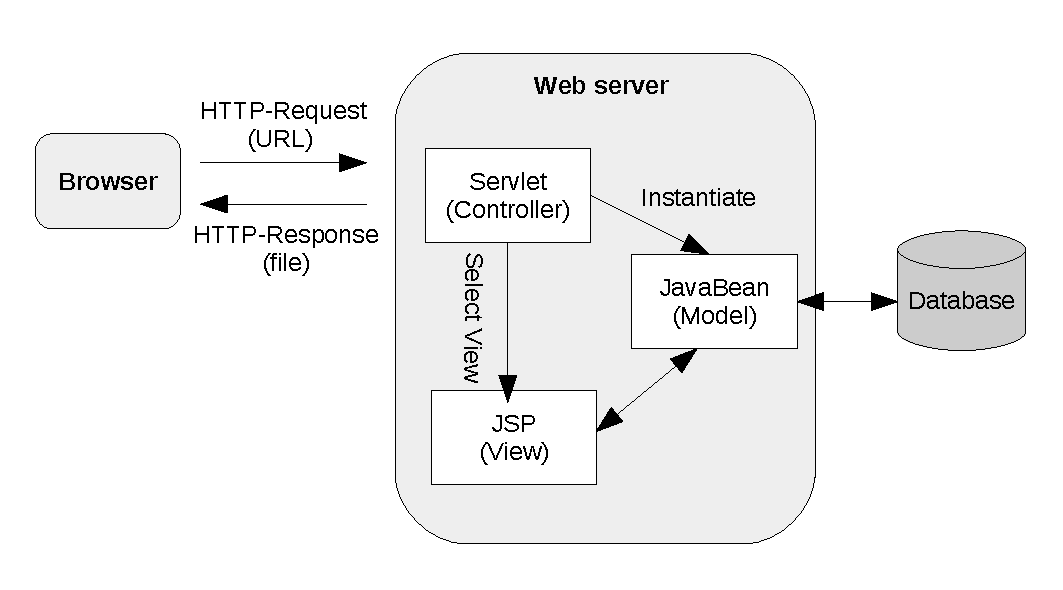
\includegraphics[width=8cm]{pics/jspMVC.pdf}}
    \caption{Model of JSP}
    \label{fig-jspMvc}
\end{figure}
\end{frame}

\begin{frame}
\frametitle<presentation>{JSP - JavaServer Pages}

  Similarly to PHP, JSPs are HTML files with embedded Java code
  
  \begin{alertblock}{But}
  Usually the code is meant as directives to display data. It should not contain logic.
  \end{alertblock}
\end{frame}

\begin{frame}[fragile]
\frametitle<presentation>{JSP - JavaServer Pages}
  \begin{exampleblock}{Example}
    \begin{lstlisting}[language=html, captionpos=b,caption={Java embedded in HTML. Taken from \cite{downey2008web}},label=lst:jsp]
        Hobby:
        <input type="text" name="hobby" 
        value="${refData.hobby}">
        <br>
        Aversion:
        <input type="text" name="aversion" 
        value="${refData.aversion}">
    \end{lstlisting}
  \end{exampleblock}

\end{frame}

\begin{frame}
  \begin{multicols}{2}
    Advantages of JSP:
    \begin{itemize}
    \item Encourages more structure
    \item Supports Java Code 
    \end{itemize}
    \vfill
    \columnbreak
    
    Disadvantages:
    \begin{itemize}
      \item Difficult to trace errors
      \item Not as good performance as PHP initially: JSPs need to be compiled
    \end{itemize}
  \end{multicols}
\end{frame}

\section{Increasing Performance}

\begin{frame}
\frametitle<presentation>{Increasing Performance}

  \begin{itemize}
    \item Number of Web users grows rapidly
    \item Expanding Web infrastructure is expensive
    \item Today's Web servers use fair scheduling 
  \end{itemize}
  $\Longrightarrow$ Possible solution: Size-based unfair scheduling \cite{schroederSize} and \cite{schorederSchedule}

\end{frame}

\begin{frame}
\frametitle<presentation>{Size-based scheduling}

  \begin{itemize}
    \item Fair scheduling: Web server partitions its resources fairly among requests ready to receive service
    \item Size-based unfair scheduling: Prioritise short requests or those with short remaining file size
    \item Claim: Expected response time of every HTTP request can be reduced and minimise number of connections\cite{schroederSize} and \cite{schorederSchedule}
    \item Apache Web server an Linux were used for measurements
    \item Implementations had to be done at kernel level
    \end{itemize}
  
\end{frame}

\begin{frame}[fragile]
\frametitle<presentation>{SRPT - Shortest Remaining Processing Time first}
  \begin{itemize}
    \item Size-based scheduling goes along with SRPT
  \end{itemize}
  
  \begin{block}{SRPT}
    Preemptive Shortest Remaining Process Time first algorithm
  \end{block}
  
\begin{figure}[h]
\centerline{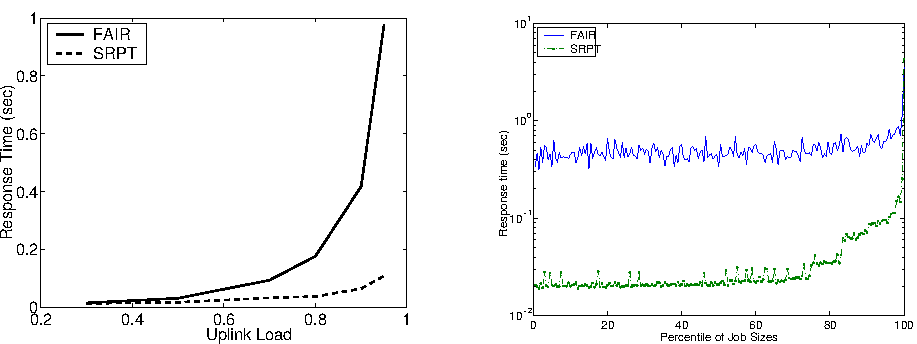
\includegraphics[width=10cm]{pics/srpt.pdf}}
\caption{(Left) Mean response time for static requests. (Right) Response time as a function of the size of the requested file, system load is fixed at
$\rho$ = 0.8. Taken from \cite{schorederSchedule}}
\label{fig-srpt}
\end{figure}

\end{frame}

\begin{frame}
\frametitle<presentation>{SRPT - Shortest Remaining Processing Time first}
Reservations against SRPT: Fear that big jobs will starve. But \cite{schorederSchedule} shows that
  \begin{itemize}
    \item Web file sizes exhibit highly variable statistical distributions with heavy tails
    \item Little if any unfairness to large requests 
  \end{itemize}
\end{frame}

\begin{frame}
\frametitle<presentation>{SRPT - Shortest Remaining Processing Time first}
  \begin{itemize}
    \item Promising approach for HTTP requests
    \item SRPT needs to know length of transaction before execution
    \item Only suitable for static files 
  \end{itemize}
  
How to increase performance for dynamic content?

\end{frame}

\begin{frame}
\frametitle<presentation>{Increasing Performance}
  \begin{itemize}
    \item LAS - Least-Attained-Service guesses the remaining service time
    \item LAS converges towards SRPT behaviour
    \item Bottleneck in processing dynamic web requests: Database backend
    \item Existing database management systems do not support effective transaction prioritisation for web based transaction workloads
    \item Lock-bound and thus need lock scheduling
  \end{itemize}
\end{frame}

\begin{frame}
\frametitle<presentation>{PAbort and NPrionher}
   \cite{McWherter} analyses following algorithms:
   
   \begin{block}{PAbort - Preemptive Abort}
      \begin{itemize}
        \item Blocking low-priority transactions gets immediately preempted
        \item Causes overhead due to rolling back and restarting
      \end{itemize}
    \end{block}
  
  \begin{block}{NPrionher}
    \begin{itemize}
      \item Grands blocking low-priority transactions temporarily high priority
      \item Causes worse high priority performance 
    \end{itemize}
  \end{block}
\end{frame}

\begin{frame}
\frametitle<presentation>{POW}

  \begin{block}{POW - Preempt-On-Wait}
 
  \begin{itemize}
    \item Preempts low-priority transactions in favour of high-priority ones
    \item But if and only if the low-priority transaction currently, or in the future, has to wait for lock
    \item Guarantees that already work done will not be lost
    \item Compromise between PAbort and NPrionher
  \end{itemize}
  
  \end{block}
\end{frame}

\begin{frame}
\frametitle<presentation>{POW, PAbort and NPrionher}

  \begin{figure}[h]
    \centerline{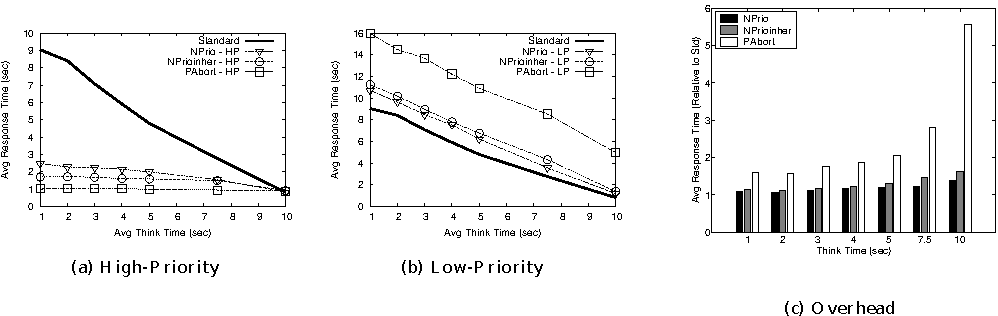
\includegraphics[width=12cm]{pics/pow.pdf}}
    \caption{Average response time for high- and low-priority transactions for \textit{POW}, \textit{PAbort}, and \textit{NPrioinher} as a function of load (a) and (b). Aggregate high- and low-priority average response time
    relative to \textit{Standard} (c). Taken from \cite{McWherter}
    }
    \label{fig-pow}
  \end{figure}

\end{frame}

\begin{frame}
\frametitle<presentation>{Increasing Performance}
  \begin{itemize}
    \item SRPT for static content
    \item POW for dynamic processing
    \item Combination of both forms appealing solution for increasing performance
  \end{itemize}
\end{frame}

\section{Conclusion}
\begin{frame}
\frametitle<presentation>{Conclusion}
  Initial Questions:
  
  \begin{enumerate}
  \item How to support development of Web sites towards more attractive and modern Web sites?
  \item How to assure high performance in the Web?
  \end{enumerate}

\end{frame}

\begin{frame}
  \begin{center}
    \huge{Any questions?}
  \end{center}
\end{frame}

\begin{frame}
  \begin{center}
    \huge{What server-side technologies did you encounter?}
  \end{center}
\end{frame}
\bibliographystyle{apalike}
\bibliography{ref}

\end{document}
